
\usepackage[T1]{fontenc}
\usepackage{mathptmx}
\usepackage[scaled=.90]{helvet}
\usepackage{courier}

\usepackage{beamerthemesplit}
\usepackage{verbatim}
\usepackage{hyperref}
\usepackage{listings}
\lstset{language=Perl,basicstyle=\footnotesize,tabsize=3,showstringspaces=false}

\title{Modern PerlCommerce}
\author[racke]{Stefan Hornburg (Racke)\\ \texttt{racke@linuxia.de}}
\date[]{Pittsburgh Perl Workshop, 8th/9th October 2011}

\begin{document}
\maketitle{}

\begin{frame}
  \titlepage
\end{frame}

\tableofcontents

\section{Modern PerlCommerce}
The theme of this conference is ``Modern Perl''.

\subsection{Modern Perl}
There isn't really a set definition what Modern Perl is about,
but I want to point the things important to us.

\begin{frame}{Modern Perl}
\begin{itemize}
\item CPAN
\item Best Practices
\item Tests
\item Separation (Modules, Plugins, Hooks, Templates)
\end{itemize}
\end{frame}

\subsection{PerlCommerce Choices}
Surprisingly there are not many choices for OpenSource PerlCommerce
software. Searching for ``cart'', ``ecommerce'' or ``shop'' on CPAN
gives you only a few results, which aren't actually very helpful.

Let's look at the possible choices for OpenSource PerlCommerce software:

\begin{frame}{PerlCommerce Choices}
\begin{itemize}
\item Interchange
\item Handel
\item Agora
\end{itemize}
\end{frame}

Interchange is around since 1995, but not in CPAN.

Handel is a framework which support AxKit, Template Toolkit 
and Catalyst.
Available from CPAN, last release a year ago.
There isn't even a mailing list.

Agora isn't modern Perl either and is around since 1999.

\begin{frame}{Status quo}
  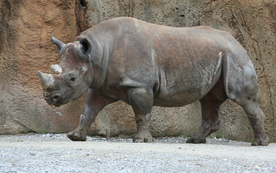
\includegraphics{rhino.jpg}
\end{frame}

\subsection{References}
\begin{frame}{References}
\begin{itemize}
\item Backcountry \url{http://www.backcountry.com/}
\item Fragnance \url{http://www.fragrancenet.com/}
\item DoS
\end{itemize}
\end{frame}

\subsection{Dancer Offerings}
\begin{frame}{Dancer Offerings}
Things supplied by Dancer or Dancer plugins:

\begin{itemize}
\item Dispatching requests
\item Session handling
\item Template engine
\item I18N
\end{itemize}
\end{frame}

\subsection{How easy can it be?}
\begin{frame}[fragile]{How easy can it be?}
\begin{lstlisting}
#!/usr/bin/env perl

use Dancer;
use Dancer::Plugin::Interchange;

sell;
\end{lstlisting}
\end{frame}

\subsection{Real World}
Running and maintaining an online shop is a challenging business
and requires constant change to stay on top of your competitors.

\begin{frame}{Real World}
\begin{itemize}
\item Marketing, SEO
\item Legal stuff
\item Interfaces
\item Design
\end{itemize}
\end{frame}

\section{API}
\subsection{Cart}
\begin{frame}{Cart}
\begin{itemize}
\item SKU, Name, Quantity, Price
\item Price > 0
\item Combines automatically
\item Multiple carts
\item Storage everywhere
\end{itemize}
\end{frame}

\begin{frame}[fragile]{Interchange::Cart Functions}
\begin{lstlisting}
$cart = Interchange::Cart->new;

$cart->add(sku => 'POM253', name => 'Pomelo',
    price => 3.00, quantity => 10);

$cart->count();

$cart->clear();

$cart->total();

$cart->subtotal();
\end{lstlisting}
\end{frame}

\subsubsection{Everything is a Cart}
\begin{frame}{Everything is a Cart}
\begin{itemize}
\item Saved Carts
\item Wishlists
\item Sets
\end{itemize}
\end{frame}

\subsubsection{Inventory Checks}
Inventory checks are pretty much limited in Interchange right now.
They are controlled by the configuration directives MinQuantityField
and MaxQuantityField:
\begin{frame}[fragile]{Inventory Check}
\begin{lstlisting}
MinQuantityField min_quantity
MaxQuantityField inventory:quantity 
\end{lstlisting}
\end{frame}
Also they are part of the standard code instead of loaded through
hooks.

\subsection{Payment}
\begin{frame}{Payment}
\begin{itemize}
\item Business::OnlinePayment
\end{itemize}
\end{frame}

\subsection{Shipping}
\begin{frame}{Shipping}
\begin{itemize}
\item Simple Shipping
\item Crazy Shipping
\item Shipping API
\end{itemize}
\end{frame}

\subsection{ACL}
\begin{frame}{Access Control}
\begin{itemize}
\item Customer Service
\item Menus
\item Backend
\end{itemize}
\end{frame}

\subsection{Forms}
\begin{frame}{Forms}
\begin{itemize}
\item Display
\item Validation
\item Storage
\end{itemize}
\end{frame}

\subsection{Backend}
\begin{frame}{Shipping}
\end{frame}

\section{Integration \& Deployment}
\subsection{Dancer}
\subsubsection{Routes}
\begin{frame}{Routes}
\begin{itemize}
\item Categories
\item Products
\item Cart
\item Checkout
\item Customer Service
\end{itemize}
\end{frame}

\subsubsection{Default Route}
Categories and products can be handled through the default route
(see
\url{http://search.cpan.org/~sukria/Dancer/lib/Dancer/Cookbook.pod#Default_route})
as alternative to defining explicit routes.

\begin{frame}[fragile]{Default Route}
\begin{lstlisting}
get qr{/(.*)} => sub {
    my ($sku) = splat;
    my $product;

    # check for existing product
    if ($product = database->quick_select('products', {sku => $sku})) {
        # display flypage
        template 'flypage', $product;
    }
    else {
        # display not found page
        status 'not_found';
        forward '404';
    }
};
\end{lstlisting}
\end{frame}
\end{document}

%%% Local Variables: 
%%% mode: latex
%%% TeX-master: t
%%% End: 
